\documentclass[11pt, a4paper]{article}
\usepackage[tmargin=1in,bmargin=1in,lmargin=1in,rmargin=1in]{geometry}
\usepackage{authblk}
\usepackage{multicol}
\usepackage{caption}
\usepackage{subcaption}
\usepackage{graphicx}
\usepackage{hyperref}
\usepackage{biblatex}
\usepackage{amsmath}
\usepackage{tabularx}


\graphicspath{ {./images/} }
\addbibresource{ref.bib}

% \DeclareUnicodeCharacter{0301}{*************************************}

\newenvironment{Figure}
  {\par\medskip\noindent\minipage{\linewidth}}
  {\endminipage\par\medskip}

\title{Cosine Similarity based TopoMap}
\author{Devarsh Patel \\
    \texttt{dp3324@nyu.edu}}
\affil{Master of Science in Computer Science, \\
    NYU Tandon School of Engineering}

\begin{document}
    \maketitle

    \begin{center}
        \textbf{Track}: Track 1 \\
        \medskip
        \textbf{Github}: \href{https://github.com/dp3324/advance-topomap}{https://github.com/dp3324/advance-topomap}
    \end{center}

    \medskip
    \begin{abstract}
        The main goal of this project is to take TopoMap\cite{harishd} one step further in terms of information computation complexity and space efficiency. It will answer many unresolved bottlenecks emerged during the initial iteration in the previous work. The point of interest for designing and developing this advanced TopoMap\cite{harishd} solution is to answer the training problem that arise in Machine Learning models because of High-Dimensional data. While using polynomial data with multiple regression model, It requires more computation time along with intensive space utilization. This project aims to minimize the dimension of the data while preserving the model accuracy and precision. The advancement of this technology can help data engineers to identify and modify the data cloud as per the requirement so that they can focus on whats more relevant that something that is unimportant.
    \end{abstract}

\begin{multicols}{2}   
    \section{Objective}
    The objective of this research paper is to optimize the conventional TopoMap\cite{harishd} algorithms so that it can efficiently define the outliners, provide better point deviation in the final representation, improve the relationship between points and their clusters.
    \section{Introduction}
    TopoMap\cite{harishd} is an advanced Multidimensional Projection (MDP) technique used for high-dimensional data, that ensures to maintain the topographical definition of data. Dealing with high-dimensional data create complex computation intensity with the increase size in dataset. To over-come this bottleneck, it is always preferred to only consider the dimension, i.e. parameters, of the dataset which has the most impact on the predicted output. This means it is more suitable to remove inert parameters or dimension of the dataset to minimize the computation time. Here where TopoMap\cite{harishd} comes, It provides better visualizations of introduced data by decreasing d-dimensional data to 2D Space vector. TopoMap\cite{harishd} is an advanced implementation of sophisticated projection techniques like Classical MDS, IsoMap, tSNE and UMAP. Most of the Multidimensional projection technique uses geographical distance as a base to define the relationship between the data points, which often results into false clustering as many times the data points in same coordinate region have significant topographical variance. Multidimensional scaling(MDS) is term coined for techniques which reduces data dimension by significant proportion. In context of projection, if a technique reduces data dimension to a point where it can be represented in 2D or 3D cartesian space, then that is called as Multidimensional Projection (MDP).

    This research paper focuses on two main aspects of original TopoMap algorithm: Euclidian Minimum Spanning Tree, and Convex Hull Alignment Algorithm. The proposed technique here uses Cosine Similarity based Minimum Spanning Tree instead of Euclidian distance. To accommodate the changes and the data type, Tree based hull alignment algorithm is proposed here. This algorithm varies from the convex hull alignment algorithm in terms of point placement in the component.

    \section{Literature Survey}
        There are many data dimensionality reduction algorithm designed to preserve the relationship between the points but most to them are based on the parameters dependents on the geographical terms. They utilizes distance based matrices like Euclidian distance to define the co-relation. They all are efficient in their own terms but comes with many limitations like leaving n-level simplexes. Many of this algorithms certainty decreases as the size of the data increases.

        \subsection{Multidimensional Scaling}
            Multidimensional Scaling or MDS is the simplest means of visualizing the similarities between the cases in the dataset. MDS uses the distance between n objects and define the cluster based on them. MDS places the n-dimensional data in 2D cartesian space such that it maintains the distance between the datapoints. There are mainly 4 type of Multidimensional Scaling algorithms.
            \subsubsection{Classical Multidimensional scaling}
                Classical multidimensional scaling also known as Principle Component Analysis (PCA), Torgerson Scaling or Torgerson–Gower scaling, is an algorithm which takes the input matrix giving the dissimilarities between the pairs of items and place them such that the loss function or strain is minimized. The strain can be defines as follows:
                \medskip
                \begin{flushleft}
                    \begin{math}
                        Strain_{D}(x_{1},x_{2}....x_{n} ) =
                    \end{math}
                \end{flushleft}
                \begin{flushright}
                    \begin{math}
                        \left(\dfrac{\sum_{i,j} (b_{ij} - x_{i}^{T}x_{j})^{2}}{\sum_{i,j}b_{ij}^{2}}\right) ^{1/2}
                    \end{math}
                \end{flushright}
                where \(x_{i}\) are the N-dimensional space vectors, \(x_{i}^{T}x_{j}\) defines the scalar product between \(x_{i}\) and \(x_{j}\) and \(b_{ij}\) are the element of matrix B.   
            \subsubsection{Metric Multidimensional scaling}
                Metric Multidimensional scaling is similar to the Classical Multidimensional scaling but it tries to minimize the Strain in the space instead of the stress.
                \begin{flushleft}
                    \begin{math}
                        Stress_{D}(x_{1},x_{2}....x_{n} ) = 
                    \end{math}
                \end{flushleft}
                \begin{flushright}
                    \begin{math}
                        \sqrt{\sum_{i \neq j=1,..,N}\left(d_{ij} - \| x_i - x_j \| \right)^{2}}
                    \end{math}
                \end{flushright}
            \subsubsection{Non-metric multidimensional scaling}
                In contrast to non classical and metric multidimensional scaling, Non-metric MDS finds both the non-parametric monotonic between the data points and the Euclidian distance between them. This data dimensionality reduction algorithm is based on isotonic regression. 

                For \(x\) denote the vector of proximities, \(f(x)\) a monotonic transformation of \(x\), and \(d\) as the point distance, then the coordinate of the points in 2D cartesian are found by minimizing the stress as follows:

                \begin{center}
                    \begin{math}
                        Stress = \sqrt{
                            \dfrac{
                                \sum{\left(f(x) - d\right) ^{2}}
                            } {
                                \sum{d^{2}}
                            }
                        }
                    \end{math}
                \end{center}
            \subsubsection{Generalized multidimensional matrix}
                This method is extension of metric multidimensional scaling which utilizes the non-Euclidian space. It allows finding the minimum-distortion embedding of one surface into another.

        \subsection{Topology-based Multidimensional Projection}
            Topology-based methods exist from a very long time when it comes to visualizing data. It has played an important role in many visualization prone domains like astrophysics, medical imaging, robotics and material science. The described TopoMap is based on the Rips\cite{rips} filtration technique. Rips filtration technique is used to topographically analysis the high-dimensional data point which also efficiently capture the homology of the manifold sampled by this data points. It also correlates to the Reeb Graph\cite{reedgraph}, which contract the cluster of similar topological definition to a single point, which result into skeleton like visualization. When it comes to discrete point cloud visualization, the Mapper\cite{mapper} is an better approach which is based on Reed\cite{reedgraph} approximation for the nearest neighbor graph.

        \subsection{Topology-based Multidimensional Projection}
            TopoMap\cite{harishd} provides an in-depth comparison to multiple Multidimensional Scaling(MDP)/Multidimensional Projection(MDP) techniques. While most of them works on geodesic distance between the data points, especially conventional Isomap, TopoMap\cite{harishd} works on homological difference between the points. IsoMap, tSNE and UMAP have many improved variation but they all does not preserve 0-cyclic groups. An Isomap variant proposed by Lee and Verleysen\cite{leeverleysen}, tears the high-dimension data into non-contractable loops which preserves manifold unfolding. 
        
        The work represented here, by considering Rips Filtration\cite{rips}, is focused on analyzing topographical distance. The TopoMap is compared to the terrain metaphors by the separation point of preserving the topological angle. It is guarantied that TopoMap preserves the connected component during filtration and result into identical 0-cyclic homology persistence diagram from the produced result and original data.
    \section{Methodology}
    The methodology proposed here is an extension to the original implementation of TopoMap\cite{harishd} to improve outliner detection, clear point deviation in the cluster, and relations between points and clusters. This focused areas in the original TopoMap\cite{harishd} are: Minimum Spanning Tree and Hull Alignment algorithm.
        \subsection{TopoMap: Original Algorithm}
        This original TopMap\cite{harishd} was implemented using Euclidian Minimum Spanning Tree and Convex Hull Alignment. It was designed and developed in C++. The overall time-complexity of this algorithm is O\(N\log{N}\alpha N\). This algorithm was divided in 2 phases: Calculate Euclidian Minimum Spanning Tree and Align components based on Convex Hull Algorithm.
        
        \begin{Figure}
            \centering
            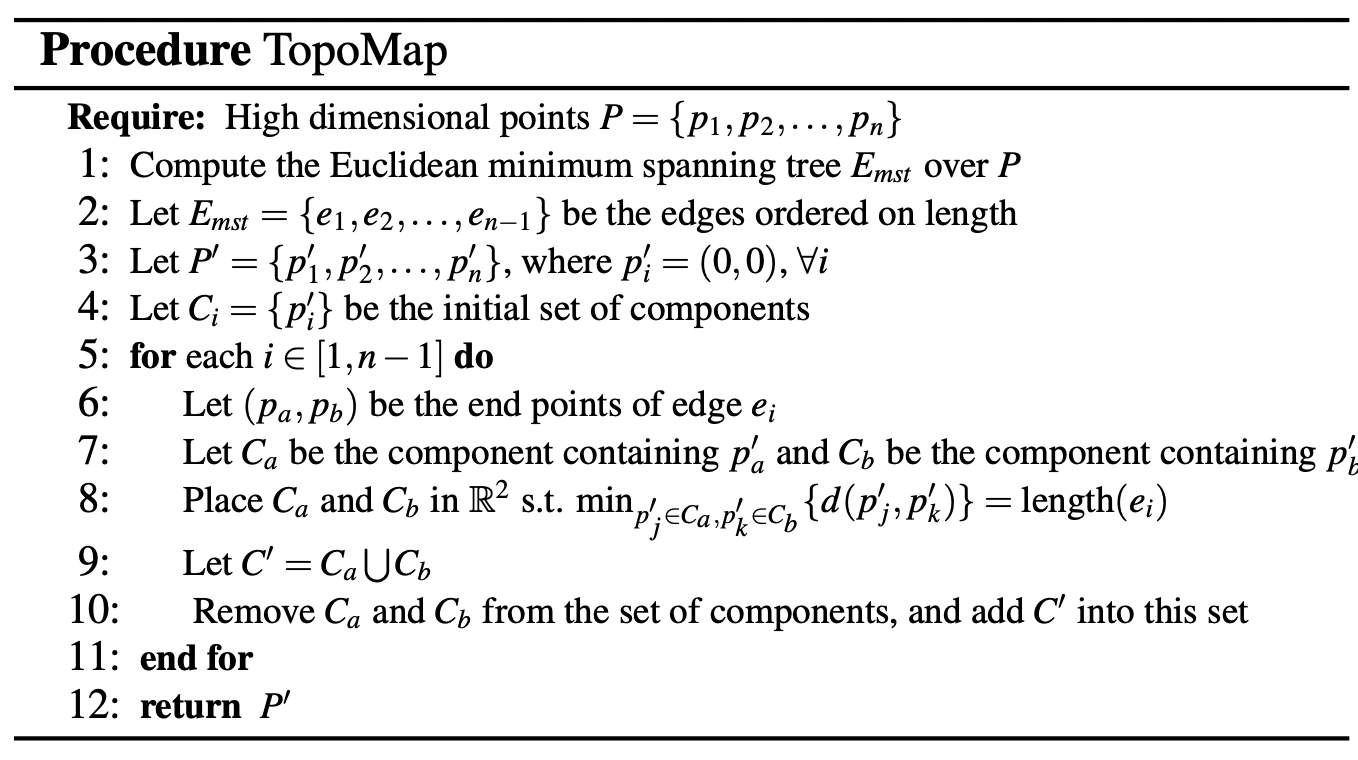
\includegraphics[width=\linewidth]{original_topomap.png}
            \captionof{figure}{Original TopoMap Implementation}
            \label{orig_topomap}
        \end{Figure}
        
        \subsection{Minimum Spanning Tree: Cosine Similarity algorithm}
        As the original TopoMap\cite{harishd} uses Euclidian distance as the base of creating Minimum Spanning Tree, It only defines the geometrical, specifically distance, relations between the data. While this method is better, it does not take point inclination into the account. The Cosine Similarity is the well know method used in Natural Language Processing, to find the similarities between two or more words. Taking the inference from this, This paper proposed changes to the TopoMap\cite{harishd} implementation by designing it using the radian angle value instead of euclidian distance. The modified algorithm is stated in Figure \ref*{cos_mst}.
\end{multicols}
\begin{figure}[t!]
    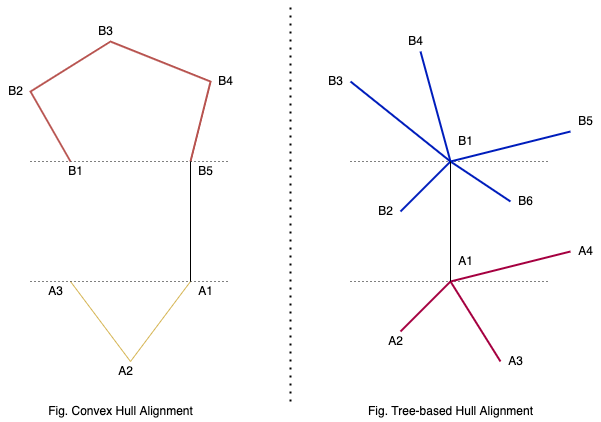
\includegraphics[width=\linewidth, height=6cm]{tree_based_hull_alignment.png}
    \captionof{figure}{Comparison between Convex Hull Alignment and Tree-based Hull Alignment algorithm.}
    \label{comparison}
\end{figure}
\begin{multicols}{2}
        \begin{Figure}
            \centering
            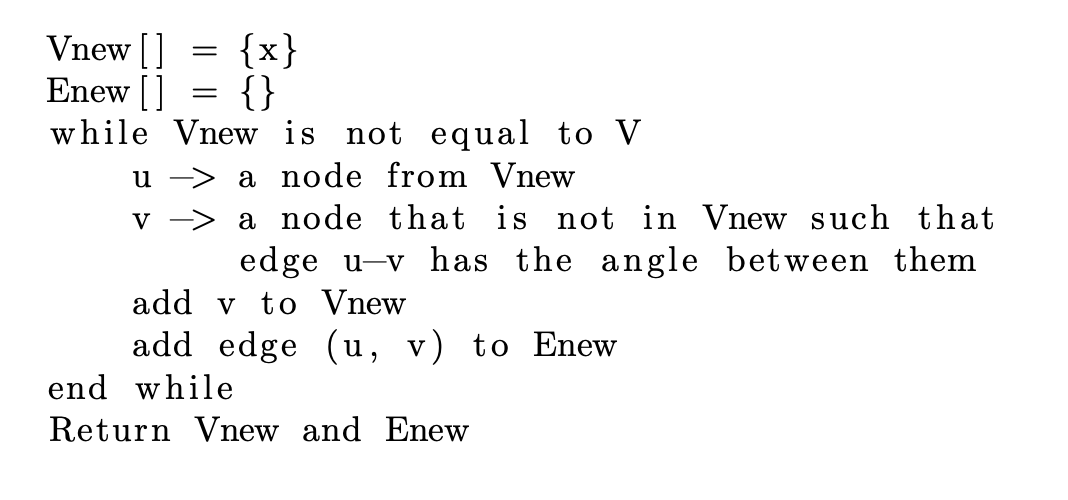
\includegraphics[width=\linewidth]{mst.png}
            \captionof{figure}{Cosine Similarity based Minimum Spanning Tree}
            \label{cos_mst}
        \end{Figure}
        \subsection{Tree-based hull alignment algorithm}
        The most important part of the original TopoMap\cite{harishd} implementation is to plot the minimum spanning tree obtained using hull alignment algorithm. These algorithm takes two points from different components containing the edge vertices and place them such that one component is shaped convex and the other one as concave as showed on left side of Figure \ref*{comparison}.Even though this provided better visualization it does not provide proper point deviation. This method can run into serious alignment issues if the size of the components increases. It can run out of joining sides. Also it should be taken into consideration that this algorithm only uses the points on the outer edge of the component to align the hull. That means that the components might not joined on the edge used. Which in turns remove the original relationship between the points and also between their clusters. While this method is useful, It can be improved if the algorithm take all the points in the component into consideration to align the hull. The proposed tree-based hull alignment algorithm uses the sum of y-values of the points in the component to decide the weight. to alight the component in the convex fashion, the algorithm minimize the weight and vice-versa for the concave fashion. The result of this improved algorithm can be seen on right side of Figure \ref*{hull_alignment}. The pseudo-code of this algorithm is shown in Figure \ref*{comparison}.

        \begin{Figure}
            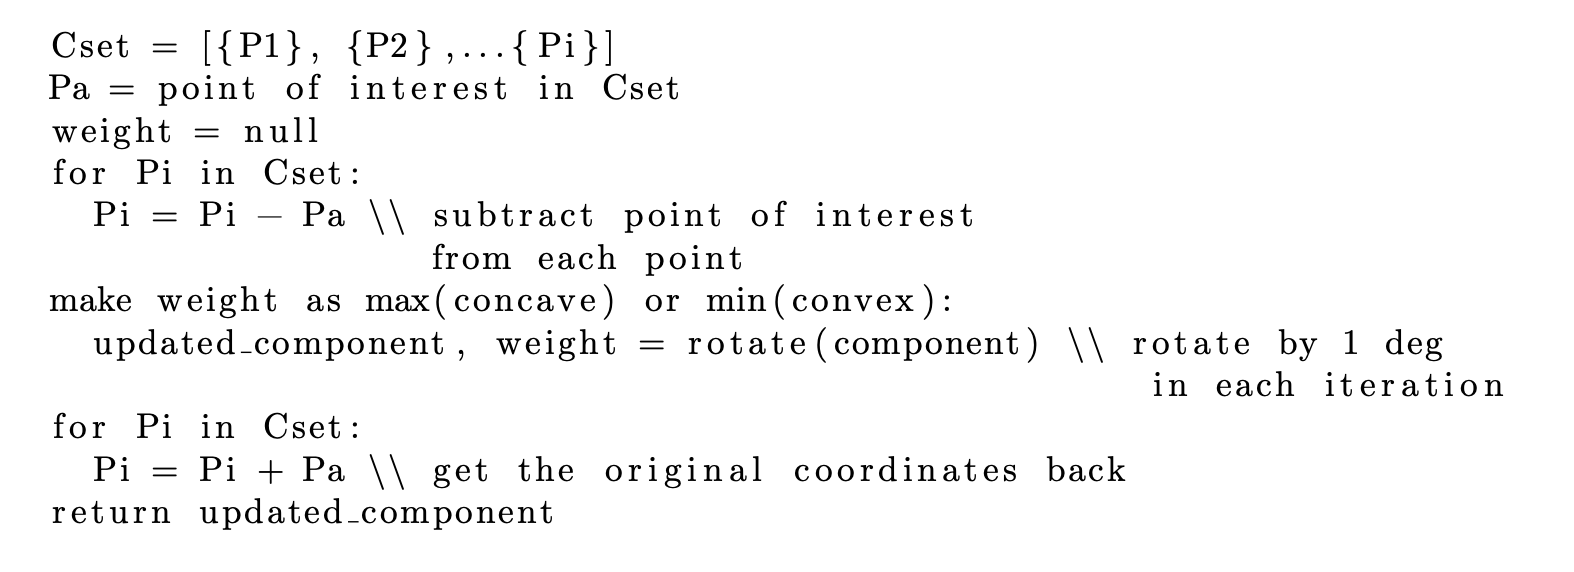
\includegraphics[width=\linewidth]{hull_alignment.png}
            \captionof{figure}{Tree-based Hull Alignment Algorithm}
            \label{hull_alignment}
        \end{Figure}

        This improved algorithm was not only able to provide better relations between the point but was also able to create improved point deviation among the points and clusters. The propose tree based hull alignment was clearly and efficiently was able to provide the relation between the points and their cluster.

        The time complexity was decreased by approximately 25\% as the space-complexity of the algorithm decreased by significant amount of approximately 10\% by increasing the complexity of calculations due to Cosine Similarity based Euclidian Minimum Spanning Tree and Tree-based hull alignment algorithm.

    \newpage
\end{multicols}

    
    \begin{figure}[h]
        \centering
        \begin{subfigure}[b]{0.3\textwidth}
            \centering
            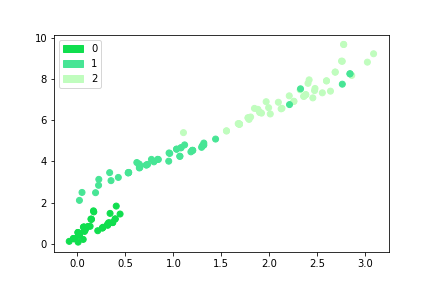
\includegraphics[width=\textwidth]{iris_euclidian_distance_1.png}
            \caption{Iris Dataset}
            \label{iris_euclid}
        \end{subfigure}
        \hfill
        \begin{subfigure}[b]{0.3\textwidth}
            \centering
            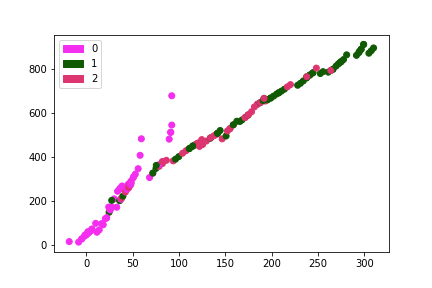
\includegraphics[width=\textwidth]{wine_euclidian_distance_1.png}
            \caption{Wine Dataset}
            \label{wine_euclid}
        \end{subfigure}
        \hfill
        \begin{subfigure}[b]{0.3\textwidth}
            \centering
            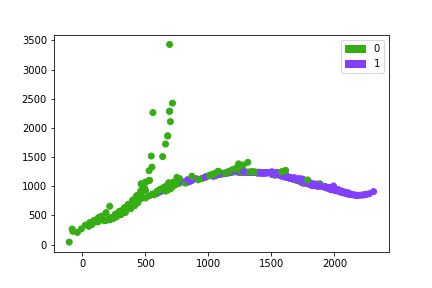
\includegraphics[width=\textwidth]{breast_cancer_euclidian_distance_1.png}
            \caption{Breast Cancer Dataset}
            \label{breast_cancer_euclid}
        \end{subfigure}
            \caption{Euclidian Distance based TopoMap}
            \label{euclid}
    \end{figure}

    \begin{figure}[h]
        \centering
        \begin{subfigure}[b]{0.3\textwidth}
            \centering
            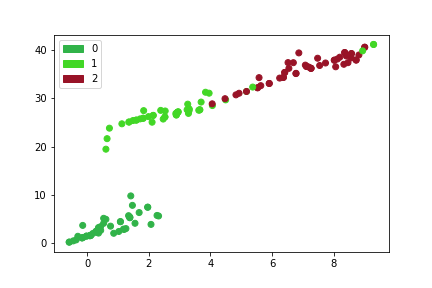
\includegraphics[width=\textwidth]{iris_angle_1.png}
            \caption{Iris Dataset}
            \label{iris_angle}
        \end{subfigure}
        \hfill
        \begin{subfigure}[b]{0.3\textwidth}
            \centering
            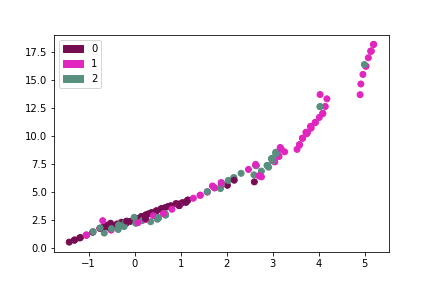
\includegraphics[width=\textwidth]{wine_angle_1.png}
            \caption{Wine Dataset}
            \label{wine_angle}
        \end{subfigure}
        \hfill
        \begin{subfigure}[b]{0.3\textwidth}
            \centering
            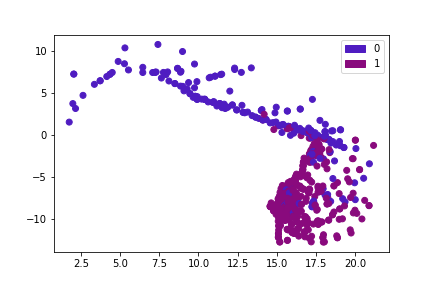
\includegraphics[width=\textwidth]{breast_cancer_angle_1.png}
            \caption{Breast Cancer Dataset}
            \label{breast_cancer_angle}
        \end{subfigure}
            \caption{Cosine Similarity based TopoMap}
            \label{angle}
    \end{figure}

\begin{multicols}{2}
    \section{Results \& Discussion} 
    Topological representation of the high dimensional data is a better option compared to the convention multidimensional scaling algorithms like Multidimensional Scaling, T-SNE, and UMAP. The algorithm proposed here was efficient optimized, scalable, and robust. This improvised algorithm of the original TopoMap\cite*{harishd} implementation provided solid proofs of data relationship preservation of both 0-cyclic and correlation based on inclination. It was tested using open-source datasets available on Scikit learn library like Iris, Wine, and Breast Cancer. 
    \begin{center}
        \begin{tabularx}{\linewidth} { 
            | >{\raggedright\arraybackslash}X 
            | >{\centering\arraybackslash}X 
            | >{\centering\arraybackslash}X
            | >{\centering\arraybackslash}X | }
            \hline
            \bf Data set & \bf \# Inst. & \bf \# Attr. & \bf \# Cls. \\
            \hline
            Iris & 150 & 5 & 3 \\ 
            \hline
            Wine & 178 & 13 & 3 \\
            \hline
            Breast Cancer & 569 & 30 & 2 \\
            \hline
        \end{tabularx}
    \end{center}
    As we can see in Fig. \ref*{euclid} and Fig. \ref*{angle}, that the angle based implementation is providing better point separation and deviation compared to Euclidian distance based minimum spanning tree on improved hull alignment algorithm. We can clearly notice that even when the data is clouded and intensive the algorithm was able to provide sufficient differentiation compared to original TopoMap\cite*{harishd} implementation.

    The overall processing and running time for both of these algorithms was 10\% less than the original algorithm of TopoMap\cite*{harishd}.



    \section{Future Scope}
    There are many improvement that can be done in this improved TopoMap\cite*{harishd} as follows:\newline\textbf{3-Dimensional Implementation}: It will be exciting to see the plotted data in 3D, as it will provide details on covered datapoints.\newline\textbf{Optimized MST}: It will be more efficient if there is a way to optimize the current minimum spanning tree by decreasing time complexity to \(O(N\log{N})\).
    \section{Conclusion}
    The interpretation of N-dimensional dataset was efficiently reduced to 2D plotting and was able to increase model training speed by almost 75\% which is more efficient when it comes to large datasets. Extensions of this algorithms will help in decreasing it deep learning models hyper-parameters and layer size.
\end{multicols}
    \newpage
    \printbibliography
\end{document}